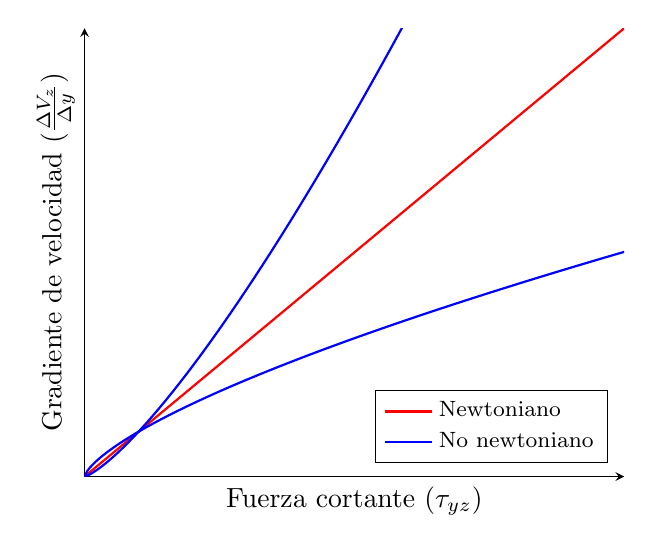
\begin{tikzpicture}
\begin{axis}[
    axis lines = left,
    ticks = none,
    xmin=0, xmax=10,
    ymin=0, ymax=10,
    xlabel = {Fuerza cortante ($\tau_{yz}$)},
    ylabel = {Gradiente de velocidad ($\frac{\Delta V_{z}}{\Delta y}$)},
    domain=0:10, 
    samples=200,
    legend pos = south east,
    legend cell align = left
]
    \addplot[thick, color=red]{x};
    \addlegendentry{\footnotesize Newtoniano}
    \addplot[thick, color=blue]{x^0.7};
    \addplot[thick, color=blue]{x^1.3};
    \addlegendentry{\footnotesize No newtoniano}
\end{axis}
\end{tikzpicture}